\documentclass[sigplan,anonymous,review]{acmart}

\usepackage{authorcomments}
\usepackage{listings}
\usepackage{algorithm}
\usepackage{algpseudocode}
\usepackage{xspace}
\usepackage{paralist}


\lstset{language=R}
\definecolor{LightGray}{rgb}{.92,.92,.92}
\definecolor{Gray}{rgb}{.3,.3,.3}
\definecolor{DarkGray}{rgb}{.5,.5,.5}
\lstset{ %
  columns=flexible,
  captionpos=b,
  frame=single,
  framerule=0pt,
  tabsize=2,
  belowskip=0.5em,
  backgroundcolor=\color{LightGray},
  basicstyle=\small\ttfamily,
  emphstyle=,
  keywordstyle=,
  commentstyle=\color{Gray}\em,
  stringstyle=\color{Gray},
  numbers=left,
  showstringspaces=false
}
\lstdefinestyle{R}{ %
  language=R,
  morekeywords={assign, delayedAssign},
  deletekeywords={env, equal, c, runif, trace, args, exp, t, all},
  breaklines=true
}
\lstdefinestyle{Rin}{ %
  style=R,
  breaklines=false
}


\newcommand{\tool}{\texttt{signatr}\xspace}
\newcommand{\numFnsCaseStudy}{20\xspace}
\newcommand{\numPkgsScaleStudy}{20\xspace}
\newcommand{\code}[1]{{\lstinline[style=Rin]!#1!}\xspace}

% For algorithmcx
\algnewcommand{\LineComment}[1]{\State \(\triangleright\) #1}
\newcommand{\DBFileSize}{287.17 GB\xspace}
\newcommand{\DBValuesRnd}{39.4M\xspace}
\newcommand{\DBValues}{39,425,582\xspace}
\newcommand{\DBNumPackagesRnd}{652\xspace}
\newcommand{\DBNumPackages}{652\xspace}
\newcommand{\DBNumFunctionsRnd}{38.1K\xspace}
\newcommand{\DBNumFunctions}{38,109\xspace}
\newcommand{\DBNumSourceFilesRnd}{17.5K\xspace}
\newcommand{\DBNumSourceFiles}{17,463\xspace}
\newcommand{\DBSourceLinesOfCodeRnd}{389.7K\xspace}
\newcommand{\DBSourceLinesOfCode}{389,740\xspace}

\newcommand{\UFTracingBudgetRnd}{5K\xspace}
\newcommand{\UFTracingBudget}{5,000\xspace}
\newcommand{\UFNumTracesRnd}{12.1M\xspace}
\newcommand{\UFNumTraces}{12,115,000\xspace}
\newcommand{\UFNumSuccessTracesRnd}{2.1M\xspace}
\newcommand{\UFNumSuccessTraces}{2,062,046\xspace}
\newcommand{\UFRatioSuccessTraces}{17\%\xspace}
\newcommand{\UFNumPackagesRnd}{78\xspace}
\newcommand{\UFNumPackages}{78\xspace}
\newcommand{\UFNumFunctionsRnd}{2.4K\xspace}
\newcommand{\UFNumFunctions}{2,423\xspace}
\newcommand{\UFNumOfCrashedRSessionsRnd}{201\xspace}
\newcommand{\UFNumOfCrashedRSessions}{201\xspace}
\newcommand{\UFNumSuccessPackagesRnd}{69\xspace}
\newcommand{\UFNumSuccessPackages}{69\xspace}
\newcommand{\UFNumSuccessFunctionsRnd}{1.2K\xspace}
\newcommand{\UFNumSuccessFunctions}{1,228\xspace}
\newcommand{\UFNumFunctionSignatrSignatureRnd}{1.1K\xspace}
\newcommand{\UFNumFunctionSignatrSignature}{1,113\xspace}
\newcommand{\UFAvgNewSignatrSignatureRnd}{707.7\xspace}
\newcommand{\UFAvgNewSignatrSignature}{707.7\xspace}
\newcommand{\UFAvgNewSignatrSignatureRatioRnd}{213\xspace}
\newcommand{\UFAvgNewSignatrSignatureRatio}{213\xspace}
\newcommand{\UFBaselineSignaturesRnd}{8.3K\xspace}
\newcommand{\UFBaselineSignatures}{8,272\xspace}
\newcommand{\UFSignatrSignaturesRnd}{787.7K\xspace}
\newcommand{\UFSignatrSignatures}{787,696\xspace}
\newcommand{\UFSharedSignatureRnd}{834\xspace}
\newcommand{\UFSharedSignature}{834\xspace}
\newcommand{\UFSharedSignatureFunctionRnd}{432\xspace}
\newcommand{\UFSharedSignatureFunction}{432\xspace}
\newcommand{\UFSignatrBaselineSignaturesRatioRnd}{95.2\xspace}
\newcommand{\UFSignatrBaselineSignaturesRatio}{95.2\xspace}
\newcommand{\UFNumMissingFunctionSignatrRnd}{1.3K\xspace}
\newcommand{\UFNumMissingFunctionSignatr}{1,310\xspace}
\newcommand{\UFNumMissingFunctionSignatrRatio}{54.1\%\xspace}
\newcommand{\UFNumFunctionSignatrSignatureRatio}{45.9\%\xspace}
\newcommand{\UFNumFunctionBaselineSignatureRnd}{2K\xspace}
\newcommand{\UFNumFunctionBaselineSignature}{2,038\xspace}
\newcommand{\UFNumFunctionBaselineSignatureRatio}{84.1\%\xspace}
\newcommand{\UFNumErrorMessagesRnd}{789.9K\xspace}
\newcommand{\UFNumErrorMessages}{789,896\xspace}

\newcommand{\TRTracingOverhead}{7.8\xspace}
\newcommand{\TRTracingFilesRnd}{3.2K\xspace}
\newcommand{\TRTracingFiles}{3,236\xspace}
\newcommand{\TRAvgTracingOverhead}{3.3\xspace}
\newcommand{\TRMaxTracingOverhead}{7.8\xspace}
\newcommand{\TRMinTracingOverhead}{1.2\xspace}
\newcommand{\TRTracingBudgetRnd}{5K\xspace}
\newcommand{\TRTracingBudget}{5,000\xspace}
\newcommand{\TRTracesSize}{353.55 MB\xspace}
\newcommand{\TRTracesReturnDbsSize}{58.39 GB\xspace}
\newcommand{\TRNumTracesRnd}{12.1M\xspace}
\newcommand{\TRNumTraces}{12,115,000\xspace}
\newcommand{\TRNumSuccessTracesRnd}{2.1M\xspace}
\newcommand{\TRNumSuccessTraces}{2,062,046\xspace}
\newcommand{\TRRatioSuccessTraces}{17\%\xspace}
\newcommand{\TRNumPackagesRnd}{78\xspace}
\newcommand{\TRNumPackages}{78\xspace}
\newcommand{\TRNumFunctionsRnd}{2.4K\xspace}
\newcommand{\TRNumFunctions}{2,423\xspace}
\newcommand{\TRNumOfCrashedRSessionsRnd}{201\xspace}
\newcommand{\TRNumOfCrashedRSessions}{201\xspace}
\newcommand{\TRNumSuccessPackagesRnd}{69\xspace}
\newcommand{\TRNumSuccessPackages}{69\xspace}
\newcommand{\TRNumSuccessFunctionsRnd}{1.2K\xspace}
\newcommand{\TRNumSuccessFunctions}{1,228\xspace}



\begin{document}

\title{\tool: A Data-Driven Fuzzing Tool for R}

\begin{abstract}

The fast-and-loose, permissive semantics of dynamic programming languages limit the power of static analyses, and so precise analysis is often achieved through running code with dynamic program analysis. 
That said, dynamic analysis is only as good as the quality and quantity of available runnable code, and relying solely on things like application test suites is fraught as they likely do not cover the full gamut of what is possible, especially in a dynamic language.
% When trying to draw broader conclusions using dynamic analysis, however, existing code is often insufficient as it does not typically cover the full gamut of what is possible in a dynamic language.
Fuzzing is an approach for automatically exercising code, and could be used to generate yet more runnable code.
However, the shape of user-defined data in dynamic languages is difficult to glean statically, limiting a fuzzer's ability to generate realistic inputs.

In this work, we propose a novel feedback-driven blackbox fuzzing approach which draws inputs from a database of values recorded from existing code.
% Unlike traditional use of fuzzing, \Ie, to discover bugs and vulnerabilities, our aim to find new \textit{successful} function invocations that can extend the scope of program analysis.
We implement this approach in a tool called \tool for the R programming language.
We present the insights of its design and implementation, and assess \tool's ability to uncover new successful function calls by fuzzing \UFNumFunctions R functions, revealing \UFSignatrSignatures (\UFSignatrBaselineSignaturesRatio times more) new unique call signatures than existing code alone.


%
% Old Abstract
%


% Dynamic analysis is often the only way to precisely analyse code written in dynamic languages as the semantics of these languages render static analyses unsound. % renders static analysis loose its imprecision to the point is becomes useless.
% Dynamic analysis, however, requires both code to run and valid inputs for said code; while one could exclusively analyze existing code (e.g., tests or examples), such code paints an incomplete picture as the permissive semantics of dynamic languages can lead to puzzling runtime behavior.
% To obtain more runnable code, one could make use of a \textit{fuzzer}, a tool to generate random inputs for functions, but fuzzing in the context of dynamic languages is tricky, as the shape of user-defined data is difficult to automatically determine ahead-of-time.

% In this work, we propose a novel feedback-driven blackbox fuzzing approach which draws function inputs from a database populated with values recorded from existing code.
% Unlike traditional use of fuzzing, \Ie, to discover bugs and vulnerabilities, our aim to find new \textit{successful} function invocations that can extend the scope of a program analysis.
% We implement this approach in a tool called \tool for the R programming language.
% We present the insights of its design and implementation, and report on an application in the context of language design.
% Concretely, we stress-test one of the proposed type system designs for R, where function types were inferred from recorded call signatures from functions tests and examples.
% Fuzzing \UFNumFunctions of those R functions, \tool generated \UFSignatrAdditionalSignatures (\UFSignatrAdditionalSignaturesRatio times) more unique call signatures in comparison to the original study.

\end{abstract}

\maketitle

\section{Introduction}
\label{sec:introduction}

Dynamic analysis is often the only way to precisely analyse code written in dynamic languages as the semantics of these languages render static analyses unsound. 
Dynamic analysis, however, requires both code to run and valid inputs for said code; to draw conclusions about a code base, one could run the existing, runnable code, \Eg, tests or examples, but such code paints an incomplete picture as the permissive semantics of dynamic languages can lead to puzzling runtime behavior.

To obtain more runnable code, one could make use of a \textit{fuzzer}, a tool that essentially tries to exercise code with random inputs. 
Fuzz testing is extremely popular and has seen widespread adoption across many different programming languages, primarily to find bugs, performance pathologies and security vulnerabilities.
However, \textit{dynamically typed} programming languages such as Python, JavaScript, and R pose unique challenges that revolve around the idea that \textit{dynamically typed code tends not to result in runtime errors}.
For instance, accessing a non-existent field of an object in JavaScript yields the value {\tt undefined} instead of crashing, and basic functions in R will readily coerce values whose types do not match (and the coercion rules depend on the function in question).
A tool that tries to run code automatically will thus have very little to go on vis-\`a-vis the correctness of the code being generated.
On top of this, the lack of static types leaves fuzzers with very little information about what types of values are expected to begin with.

% Value types are hard to come by.
Another important challenge facing fuzzing in the context of dynamic languages is the difficulty in generating complex values automatically.
In a statically typed language like Java, the shapes of user-defined objects can be inferred from a static class definition, and this not always possible in, \Eg, dynamic prototype-based inheritance in JavaScript, or dynamic object definition in R.
This limits a fuzzer's ability to generate realistic and interesting inputs.
% Thus, an effective fuzzer would need to be manually equipped with the ability to create values of these complex types, which places an undue burden on developers.

% In this paper, ...
To get around this, we propose a general-purpose approach for fuzzing that relies on a database of values observed during the execution of real code.
We develop a tracer that collects information about function calls and values observed during code execution, and this information is stored in a database with an expressive query API.
Our fuzzing approach relies on this database to generate new function calls using the recorded values.
This approach is implemented in a tool called \tool for the R programming language.

% Retrofitted.
To help show that the approach discovers new and interesting calls to functions, we inferred types for all of the successful calls \tool uncovered.
As R lacks static types, we use the {\tt contractr} type inference tool from the Turcotte et al. paper proposing a type annotation language for R~\cite{turcotte2020designing}, wherein function types were inferred from recorded calls in R package test, example, and vignette code (we define a function type inferred in this way as a \textit{call signature}).
Fuzzing \UFNumFunctions of those R functions, \tool generated \UFSignatrSignaturesRnd (\UFSignatrBaselineSignaturesRatio times) new unique call signatures compared to the original study.

% As a use case for our tool, we argue that a general-purpose fuzzer can aid data-driven retrofitted type system designers by providing them with unexpected but valid inputs for existing functions.
% We develop an approach for synthesizing the results of fuzzing into a type signature for a function, entirely parameterized over a type system expressed as (1) a function to infer the type of a value, and (2) a function to determine if one type is a subtype of another.


In summary, the contributions of this paper are:
%
\begin{inparaenum}[(1)]
    \item a novel fuzzing technique relying on a database of observed values;
    \item an implementation of this approach in a tool called \tool for the R programming language; and
    \item a use case for \tool where it is used to generate many yet unseen, successful inputs for thousands of R functions.
\end{inparaenum} 

% Using the tool, we generate a value database \TODO{DB stats} and use it to fuzz trace types for \TODO{experiment stats}.
% We find \TODO{result stats}.
% %
The tool is open source and is available online alongside the data set used for this paper.

\section{Background and Related Work}
\label{sec:background}

\paragraph{Related Work}

In this paper, we will propose an approach to fuzzing where no input is required from the programmer, and automatically discovers how the function or program under study should be called.
There are myriad fuzzing tools and approaches, e.g., \emph{Randoop}~\cite{pacheco2007randoop} is a feedback-driven random test generation tool for Java, though the technique underpinning it is universally applicable.
Essentially, sequences of method calls are generated to test classes, and randomly generated arguments for these calls are used in two ways: for primitives, a random value is selected from a predefined, but user-extensible list, and for reference types a value is selected at random from those which have been seen, and if none are available then {\tt null} is selected.
While this technique is effective at generating tests involving non-trivial objects that are built up from a number of method calls, these objects are uncommon in data science languages, where the challenge is generating realistic data.
\emph{QuickCheck}~\cite{quickcheck} is a tool originating in the Haskell world that helps with property-based testing.
While it can generate random program inputs, the strategy of how the random inputs are constructed need to be specified.
In R we do not have any type information about function parameters neither we know the shape of the values except for the primitive types.
American Fuzzy Lop (AFL)~\cite{afl} is a state-of-the-art industrial fuzzer; AFL takes a program and one example file as input, calls the program with the input, and then uses a variety of heuristics to transform the input and fuzz the program. The aim of AFL is to find defects, looking for edge cases.
Our approach on the other hand looks for calls that do not crash the program, but rather discovers new acceptable input.

\paragraph{The R Programming Language}

We will present a fuzzing tool called \tool for the R programming language.
R sports an unusual mix of language features making it a challenging target for
tooling~\cite{morandat2012evaluating}. 
Some major challenges include:

\begin{compactitem}[$-$]

\item R does not have type annotations or a static type system, so there is very little to suggest what are expected arguments or return values.
% This means there is nothing to suggest what the expected arguments or return values of a function could be, and thus there is little to guide test generation.

\item Primitive values (booleans, integers, doubles, complex numbers, and character strings) each have a separate ``NA'' value indicating that data is ``not available''--some operations fail on these NAs.

\item Values are automatically and silently coerced from more specific types to more general types, and each function coerces its parameters as it sees fit.

\item Most values are vectors or lists, and can be annotated by key-value pairs called \textit{attributes}. 
These annotations, coupled with reflection, are the basic building blocks for many advanced features of R. 
For example, the S3 dynamic dispatch mechanism is based on the class attribute of a value.
(In fact, R has multiple different object systems but S3 is the most widespread one.)
There is not description of a shape of an S3 object, it is simply a value with \code{class} attribute denoting its classes as a vector of character strings (a value can have multiple classes).

% I don't think we need promises.
% \item All expressions are evaluated by-need, thus the call \code{f(a+b)}
%     contains three delayed sub-expressions, one for each variable and one for
%     the call to plus. This means that R does not pass values to functions but
%     rather passes unevaluated promises (the order of evaluation of promises is
%     part of the semantics as they can have side effects). These promises can
%     also be turned back into code by reflection.

\item R has a copy-on-write semantics for shared values. A value is shared if
    it is accessible from more than one variable. This means that side effects
    that change shared values are rare. This gives a functional flavor to large
    parts of R.

 \item The primary abstraction in R is a function.
\end{compactitem}

% Types for R.
There has been some effort to develop a static type system for R.
Turcotte et al.~\cite{turcotte2020designing} proposed a simple type annotation language for types at the level of functions, inspiring themselves from a corpus analysis of 400 R packages.
As part of our assessment of \tool, we will run it on the functions in this corpus to demonstrate the many novel and unexpected ways functions can be called.


% \subsection{Test Generation for Dynamic Languages}

% Many of the aforementioned techniques rely on static function parameter types in creating values with which to call a function, and dynamic languages do not have static type information.
% For example, \emph{LambdaTester}~\cite{lambdatester} focuses on test generation for higher-order functions in JavaScript; a discovery phase is required to identify which parameters are expected to be callbacks, and all other, non-callback arguments are generated in a similar manner to \emph{Randoop}.
% Further work on \emph{Nessie}~\cite{arteca2022nessie} expanded upon the approach presented in \emph{LambdaTester} to generate tests for asynchronous callbacks using sequencing and nesting.
% Other work on fuzzing deep-learning libraries in Python~\cite{wei2022free} explicitly cite Python being a dynamic language as a challenge for test generation; an important part of the pipeline in the paper is inferring types for function parameters by running existing code.

\section{Approach}
\label{sec:fuzzy}

There are two main phases to the approach:
%
\begin{inparaenum}[(1)]
\item \emph{recording}, where R code is run and function arguments and return values are recorded in the value database, and % records each function invocation into the value database (\sxpdb), and
\item \emph{fuzzing}, where values are drawn from the database as input to R functions. 
\end{inparaenum}
%
% The tool is meant to be run as a part of a data pipeline that analyzes a corpus of code.
This is pictured in Figures~\ref{fig:sxpdb-pipeline} and \ref{fig:fuzz-pipeline} for the recording and fuzzing phases respectively.

For the recording phase (Fig.~\ref{fig:sxpdb-pipeline}), runnable code is extracted from examples and tests in R packages into R scripts.
Next, in parallel, the scripts are run, and all unique function arguments are recorded into the database, called the \sxpdb.
Finally, all the databases are merged into one and duplicate values are discarded.
R OpenSci targets~\cite{landau2021_targets} is used for orchestration, but any generic batch scheduler will do.

As for the fuzzing phase (Fig.~\ref{fig:fuzz-pipeline}), a list of functions to fuzz as well as a \sxpdb are taken as input, and the functions are fuzzed in parallel.
The output of the fuzzer is a list of successful function calls, where a successful call is defined as one that generated no warnings, errors, and did not cause R to crash.
The fuzzer relies on hooks before and after function execution: the hook before invocation allows the fuzzer to process inputs, and the hook after allows errors to be signalled and handled and the return value to be processed.
The after-invocation hook can also be used to expand the feedback given to the fuzzer.
% In dynamic analysis, we are often interested in much finer information about the function execution than simply start and end.
% For example, for the call signature inference use case, we would like to know if any of the function arguments was coerced to another type or if there was a method dispatch on it.
% This is supported via instrumentation.
Concretely, the fuzzer runs the functions using \emph{R-dyntrace}, an extended R virtual machine that supports attaching callbacks to various runtime events~\cite{goel2019}.
If a user would like to plug their own dynamic analysis directly into the pipeline, the can do so by using the 40 runtime events exposed by \emph{R-dyntrace}.

% \AT{I'm surprised to see dynamic analysis talked about here.
% Besides, the fuzzing itself isn't really parameterized over an analysis, but users would have the option to do that.}
% The fuzzer (Fig.~\ref{fig:fuzz-pipeline}) is parameterized by the concrete dynamic analysis of interest.
% The approach relies on hooks before and after function execution, allowing inputs to be preprocessed, output to be processed, and errors to be caught.
% % There are two main hooks: before a function is called allowing one to preprocess the input, and after the function is done executing allowing one to process the output or error depending whether the call was successful or not.
% The after-invocation hook can also provide feedback to the fuzzer, beyond signalling success or failure.
% \AT{Is the following critical to the fuzzer? I don't know that it belongs here, even if it is interesting.}
% In dynamic analysis, we are often interested in much finer information about the function execution than simply start and end.
% For example, for the call signature inference use case, we would like to know if any of the function arguments was coerced to another type or if there was a method dispatch on it.
% This is supported via instrumentation.
% The fuzzer runs the functions using \emph{R-dyntrace}, an extended R virtual machine that supports attaching callbacks to various runtime events~\cite{goel2019}.
% The dynamic analysis can therefore use one of the 40 runtime events to get the necessary insights (including dispatch and coercion).

Since R can crash (and did in our experiments, \Cf Section~\ref{sec:assessment}) and we do not want to lose partial results, each instance of the fuzzer consists of two processes:
One worker doing the fuzzing, and supervisor that can re-spawn the worker if it dies.
Furthermore, we run the fuzzing isolated in a container as calling arbitrary code with "random" values could have dire consequences.

The tool consists of three standalone components: \code{argtracer}, the tracer responsible for running the R code and recording function invocation, \code{sxpdb}, the value database, and \code{generatr}, the fuzzer responsible for generating inputs.
Technically, they are R packages written in combination of R and C++.

\begin{figure}
    \centering
    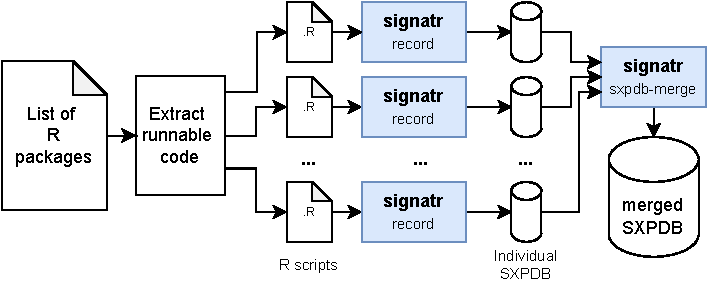
\includegraphics[width=\columnwidth]{code-and-figures/sxdb-pipeline.pdf}
    \caption{
    Recording pipeline.
    % Runnable code snippets are extracted from an input list of R packages.
    % These snippets are fed in parallel to the {\tt sxpdb-create} part of \tool, which picks out values and metadata related to them (e.g., the origin of the value). 
    % This creates a number of disparate databases that are merged into one database, which is referred to as the {\tt sxpdb}.
    }\label{fig:sxpdb-pipeline}
\end{figure}

\begin{figure}
    \centering
    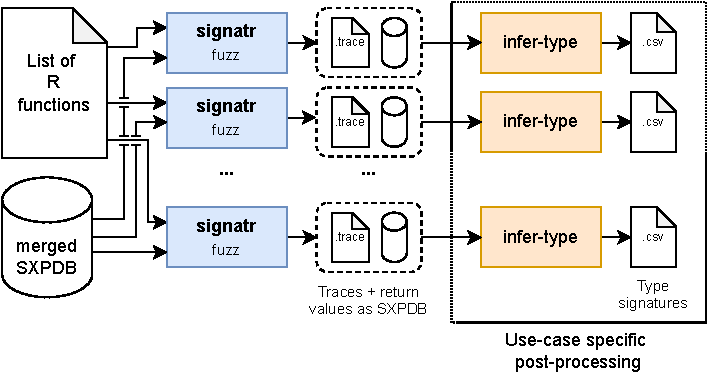
\includegraphics[width=\columnwidth]{code-and-figures/fuzz-pipeline.pdf}
    \caption{
    Fuzzing pipeline.
    % The {\tt sxpdb}, along with a list of R functions to fuzz, is input to the fuzzing phase of \tool.
    % The fuzzing phase fuzzes each of the functions w.r.t. the {\tt sxpdb}, which results in a collection of execution traces; these execution traces are fed to the typing phase of \tool, which infers types for arguments and outputs a list of unique call signatures.
    }\label{fig:fuzz-pipeline}
\end{figure}

\subsection{Tracer}\label{sec:argtracer}

The tracer is built on top of aforementioned \emph{R-dyntrace}.
The two main runtime events we use are a function exit, where all arguments are captured and stored, and a context jump, which is necessary to keep the call stack healthy.
The R interpreter uses long jumps for loops control flow, return statements and error handling.
In the case of long jump, the exit hook is ignored, so to make sure that we do not lose any function exits we maintain our version of R call stack.

When the tracer sees a call, it only sees a pointer to an R closure.
% When we see a call, we only get a pointer to R closure.
The function name and the package that contains the actual function can only be found by looking at the currently loaded namespaces and the symbols they contain.
Because of this, the tracer eagerly builds an index of package and function names when namespace functions are loaded (note: package loading in implemented in R).
% I don't think this is necessary to say.
% The fact that R is implemented in a mixture of R and C requires that we maintain a black list of R calls that are connected to R internals.
% Overall, we ignore 70 functions that are used for namespace loading and manipulation, and reflection.

Regarding performance, there is \TRMinTracingOverhead --- \TRMaxTracingOverhead (\TRAvgTracingOverhead on average) slowdown when running the R code with tracing enabled (based on the running / tracing \TRTracingFiles R scripts recording 8.2M unique values of 3.2GB size).
The main cost comes from value serialization (\Cf Section~\ref{sec:sxpdb}).
The tracer is written in 600 lines of C++ code.

\subsection{Database of Values}\label{sec:sxpdb}

The database is hand-written in order to (1) leverage some domain-knowledge of R values and store them efficiently, and (2) optimize it for the types of queries supported by the query API.
It is implemented in C++ with an R API (in 4.5K lines of C++ code and 1.5K lines of R code).

\paragraph{Storage}

The database stores only unique values.
We use XXH128, a 128bit hashing algorithm\footnote{Fast non-cryptographic hash algorithm, \Cf \url{https://cyan4973.github.io/xxHash/}} for uniqueness, in combination with a hashtable based on RobinHood hashing\footnote{\url{https://github.com/martinus/robin-hood-hashing}}.
While the hashing is fast, it works on an array of bytes so we need to lower R values into a binary format.
R provides a binary serialization format XDR\footnote{\Cf \url{https://cran.r-project.org/doc/manuals/r-release/R-ints.html\#Serialization-Formats}}, but it is costly. We also need to strip the serialization of sources of non-determinism related to character encoding.
Since there is a large number of values being pushed to the database in an average recording session, we try to avoid the serialization as much as possible.
For this we use the \emph{trace} bit that is part of the R value header\footnote{A bit in the \code{SEXP} C struct that represents R value. \Cf \url{https://cran.r-project.org/doc/manuals/r-release/R-ints.html\#Rest-of-header}}.
If it is not set, then it is a fresh value so we serialize it, compute its hash, store it into the database and set the trace bit.
If it is set, we have seen it before, but in spite of R's copy-on-write semantics, values can actually be modified in place until they are aliased, thus we need to check whether or not a value has been shared, and if not then we serialize and check its presence using the hash.


Next to the value itself, the database also store metadata about the value and its origin (the package, function and argument name).
We also store a unique call id for each sequence of argument values coming from the same call to reproduce the calls that were recorded by the tracer.

The database maintains tables for the hashes, runtime metadata (e.g., how often a value was seen), static metadata, origins, call ids, and class names. 
Variable length data, such as the serialized values, are stored in a combination of 2 tables, one giving an offset into the other table which holds the size of the value and the value itself. 
Origin strings and class names are interned, i.e., each unique string is stored separately, and referred to by pointer. 
Search indices are built using fast compressed bitsets~\cite{chambi2016better}.
The database supports all R values except external pointers.
Environments and closures (which contain environments) were not stored in the database during our experiments since they dramatically increased the size, though the database can store them.

Finally, opening the database in \textit{read mode} only loads metadata and retrieves actual values from disk on demand, making it possible to query larger-than-memory databases.

\paragraph{Queries}

% Can relax on: "na", "length", "attributes", "type", "vector", "ndims", "class"
The database provides a convenient query API.
Values can be queried based on: their {\tt typeof}-type, their class, the presence of NAs, the number of attributes, if the value is a vector or scalar, the dimensions (for tabular data), and length of the value (for vector data).
% Importantly, the database provides a convenient query API: i.e., one may sample values randomly from the database according to some parameters, such as the type \PB{Should we be more precise?}, or by providing an example value on which some characteristics (again, such as the type) can be relaxed.
The database can be queried for a random value with the desired metadata (e.g., a vector of integers of length 10), or can be queried by providing an existing value along with a list of search parameters to be relaxed (e.g., query the database for a value similar to {\tt 42}, but relax on the length). 
A custom R predicate can also be used to filter desired values.

\subsection{Fuzzing Technique}

The database of values is at the core of the fuzzing approach, which is similar in spirit to mutation-based fuzzing (where instead of mutating arguments to previous calls, new argument values are selected based on previous ones).

The core of fuzzing is to generate new calls to a function $f$, and the process of choosing arguments to construct these calls is depicted in Algorithm~\ref{alg:arg-sel}.
In addition to the function $f$ and value database $db$, the algorithm considers how many query parameters to relax on ($numRelax$), as well as all of the previously seen successful calls to $f$ ($succs$).
For each parameter $p$ of $f$, the algorithm determines which parameters to relax on (this may change from one iteration to the next), finds all values that inhabited $p$ in successful calls to $f$, chooses one such value $v$, and queries the database for a value similar to $v$ in all respects, save for the parameters that are being relaxed this time.
Note: if no successful calls to the function have been observed, random values for parameters can be chosen.

The fuzzing approach itself is depicted in Algorithm~\ref{alg:fuzzer}.
First, the collection of already known successful calls to $f$ is obtained from the database $db$.
The main idea of the approach is to start by selecting new arguments essentially at random by querying the database and relaxing on many parameters, and gradually reduce the number of parameters being relaxed as the fuzzer progresses.
Concretely, the number of parameters being relaxed is reduced every $tick$, which is determined by dividing the total fuzzing budget by the number of parameters that can be relaxed ($numRelaxParameters$).
The function $f$ will be fuzzed for as long as the budget allows, and initially all database parameters will be relaxed.
Arguments for a new call to $f$ are generated through the approach depicted in Algorithm~\ref{alg:arg-sel} ($getNewArgs$), the call is performed, and the results are saved in $res$.
If there were no errors, warnings, or crashes, then the successful call is added to the list of successful calls $succs$, and iteration continues until the budget is exhausted.

\begin{algorithm}
\caption{Selecting Arguments for New Call}\label{alg:arg-sel}
\begin{algorithmic}[1]
\Procedure{getNewArgs}{$f,numRelax,db,succs$}
\State{$params \gets getParameters(f)$}
\For{$p$ in $params$}
\LineComment{relax on $numRelax$ parameters}
\State{$relax \gets pickSome(relaxParameters, numRelax)$}
\LineComment{get all values that $p$ had in successful calls to $f$}
\State{$seed \gets getArgsFor(p, succs)$}
\LineComment{choose one at random}
\State{$v \gets pickOne(seed)$}
\LineComment{sample a similar value from the database}
\State{$args[p] \gets sampleSimilar(v, db, relax)$}
\EndFor
\State \textbf{return} $args$\Comment{the args for the new call}
\EndProcedure
\end{algorithmic}
\end{algorithm}

\begin{algorithm}
\caption{Fuzzing}\label{alg:fuzzer}
\begin{algorithmic}[1]
\Procedure{fuzzWithDB}{$f,db,budget$}
\State $succs \gets getSuccessfulCalls(f, db)$
\State $tick \gets budget / numRelaxParameters$
\State $relaxThisTime \gets numRelaxParameters$
\State $i\gets 1$
\While{$i\not=budget$}
\LineComment{gradually relax on fewer parameters}
\If{$i \bmod tick = 0$}
\State $relaxThisTime \gets relaxThisTime - 1$
\EndIf
\State{$args \gets getNewArgs(f,relaxThisTime, db, succs)$}
\State{$res \gets call(f, args)$}
\LineComment{add successful call to $succs$}
\If{no warnings, errors, crashes in $res$}
\State{$succs \gets succs + res$}
\EndIf
\State $i\gets i+1$
\EndWhile\label{endfuzzloop}
\State \textbf{return} $succs$\Comment{the successful calls to $f$}
\EndProcedure
\end{algorithmic}
\end{algorithm}

% \subsection{Use Case: Typing Successful Traces}
%
% To help show that this fuzzing approach uncovers interesting calls, we inferred types from the resulting successful calls $succs$.
% As R has no static type system, we use the type system proposed by Turcotte et al.~\cite{turcotte2020designing} by utilizing their {\tt contractr} type inference tool.
% % This is the stage where a user can define their type system, which is input as two functions: one to infer the type of some value $v$, and another to take two types $t_1$ and $t_2$ and judge whether or not they can be simplified (e.g., determine if $t_1$ is a subtype of $t_2$, $t_1 <: t_2$).
% This helps determine the set of \textit{unique} call signatures for a function, as two calls with different values that have the same type can be collapsed at this stage.
% For example, say the identity function {\tt id} was called with {\tt 4} and {\tt 2}; the types of each of those calls is $int \rightarrow int$, and so they would be collapsed together. 
%
% The fuzzing approach is implemented in a tool called \tool, written in R and C++, and is available as an R package.

\section{Assessment}
\label{sec:assessment}

We used \tool to stress-test one of the proposed type system designs for R~\cite{turcotte2020designing}.
The type system was designed empirically, with the help of a dynamic program analysis that inferred function signatures from the types of values observed while running extracted code from R packages.
In a nutshell, a type was inferred from each call to a function, and these types were unified into a single function type, and the more unique successful calls there are, the more precise the inferred signature---the types inferred from successful calls are referred to as \textit{call signatures}.
It would be therefore interesting to see \emph{how many additional successful calls can \tool generates?}

We ran all of our experiments on two Ubuntu 18.04 servers, each with a 72 core Intel Xeon 6140 2.30GHz processor and 256GB of RAM.

\paragraph{Recording}

First, we created a \sxpdb for the fuzzer.
For this we used the extracted runnable code from the same corpus as the original study which consists of \DBNumSourceFiles R scripts containing \DBSourceLinesOfCodeRnd lines of code (excluding comments and new lines).
The database was generated in 16 hours and occupies \DBFileSize of disk space.
It contains \DBValuesRnd unique values recorded from \DBNumCallsRnd calls to \DBNumFunctionsRnd functions in \DBNumPackages packages.
Figure~\ref{fig:argsdb-value-distribution} shows the distribution of main value types.
The vast majority of values are vectors and matrices of real numbers which is unsurprising as R is mostly used for numerical computing.
That said, many of them, 47.2\%  contain \textit{attributes} which is what makes them interesting, as attributes add semantic meaning.
The next big group are lists, which can be divided into two groups, data frames (two dimensional, column-major structure representing observations) and records.

\begin{figure}
    \centering
    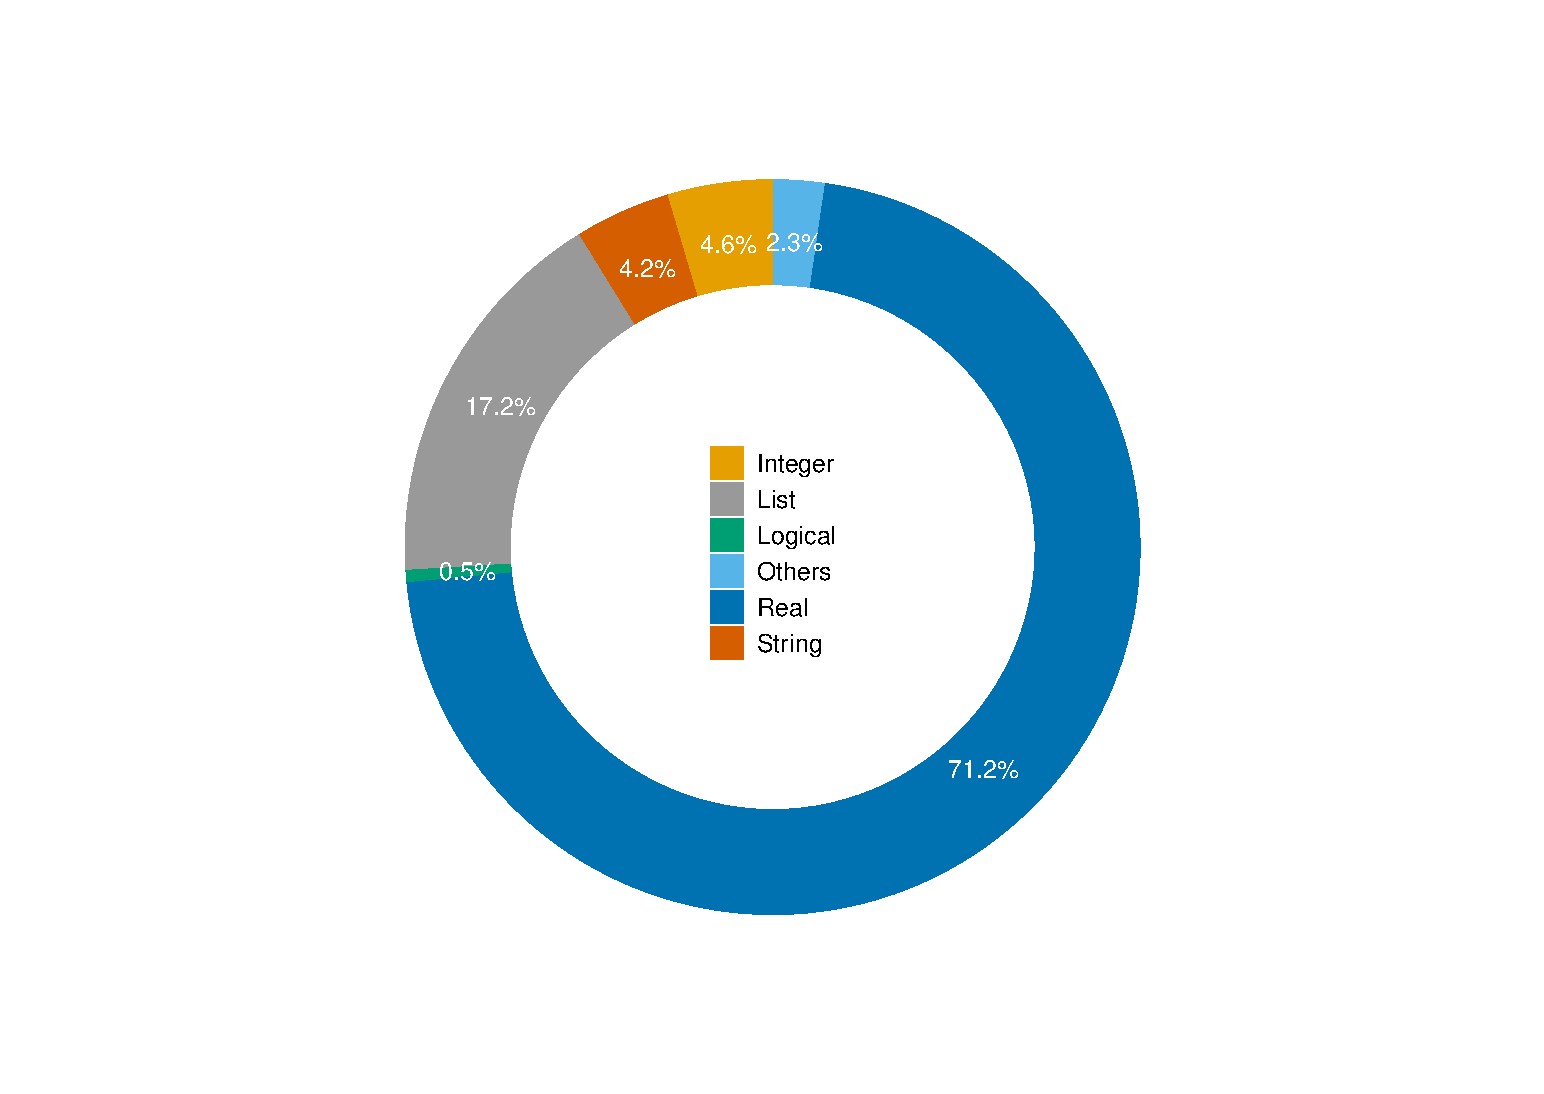
\includegraphics[width=.6\columnwidth]{code-and-figures/argsdb-value-distribution.pdf}
    \vspace{-3mm}
    \caption{The \sxpdb value type distribution}
    \label{fig:argsdb-value-distribution}
\end{figure}

\paragraph{Fuzzing}

Armed with this database, \tool fuzzed \UFNumFunctions functions from \UFNumPackages packages, a subset of the original corpus, in \UFTracingTime.
Each function was run \UFTracingBudget times, with 64 functions being fuzzed in parallel.
In total, \UFNumTracesRnd calls were made, and out of that, \UFRatioSucesssTraces were successful, resulting in \UFNumSuccessTraces traces of \UFNumSuccessFunctions functions coming from \UFNumSuccessPackages packages.
The vast majority of errors were exceptions, but in \UFNumCrashedRSessions cases, the R process crashed.
While the aim of this work is not bug finding, we have investigated one such crash in \code{stringi}\footnote{A sting processing library, one of the most downloaded package in R.}, and found that it was caused by memory corruption by large input.
The issue was reported, acknowledged and fixed.

The results of fuzzing is shown in Figure~\ref{fig:call-signatures}.
For \UFNumFunctionsSignatrSignatrue functions (\UFNumFunctionsSignatrToCorpusSignatureRatio), the fuzzer managed to generate over \UFSignatrSignaturesRnd new unique call signatures (on average \UFAvgNewSignatrSignature per function).
In comparison, recording calls from the extracted runnable code covers \UFNumFunctionsBaselineToCorpusSignatureRatio functions\footnote{The examples and tests extracted from R packages do not usually cover the full package.} generating \UFOnlyBaselineSignatures unique call signatures.
Thus we get \UFSignatrBaselineSignaturesRatio times more call signatures via fuzzing.
Fuzzed signatures overlapped in only \UFSharedSignatures cases, in \UFSharedSignatuesFunctions functions.
The reason that \tool failed to generate a single successful call for \UFNumMissingFunctionSignatr functions is because they require a very specific shape of one or more of its arguments, or the arguments depended on one-another.
As an example of the latter case, certain functions from the {\tt dplyr} data manipulation package required a data frame alongside an unevaluated expression made up of column names from the data frame. 
The functions that use non-standard scoping, manipulating arguments as unevaluated expressions and evaluating them in custom environments, are problematic.
In some cases the error message could have been used as a feedback to the fuzzer (and we plan to address it in the next iteration), but this is not easy to generalize.
% During fuzzing, we recorded \UFNumErrorMessagesRnd distinct errors and the vast majority are user-defined errors that only make sense in particular context.
% Another issue is with functions that use non-standard scoping, the R ability to allow functions to capture unevaluated expression passed to its arguments and evaluate it in custom environment.

Finally, we looked at the code coverage.
Using the \code{covr} package\footnote{The only tool for R code coverage, \Cf~\url{https://covr.r-lib.org}}, we managed to compute pairs of line coverage of R source code for \UFNumFunctionsWithBothCoverage functions, one using the fuzzed calls and the other using the traced calls.
The reason for the missing functions is failure in \code{covr} and the failure in repeating the recorded calls (in both fuzzed and trace ones).
In \UFBetterCoverage functions, the calls generated by the  tool increase the code coverage, on average by \UFBetterCoverageMean.

\paragraph{Summary}

\tool uncovers many interesting calls to functions beyond what tracing uncovers alone, particularly for highly polymorphic functions.
Together, existing and generated calls yields a wealth of interesting, runnable code.

% how often R crashed

\begin{figure}
    \centering
    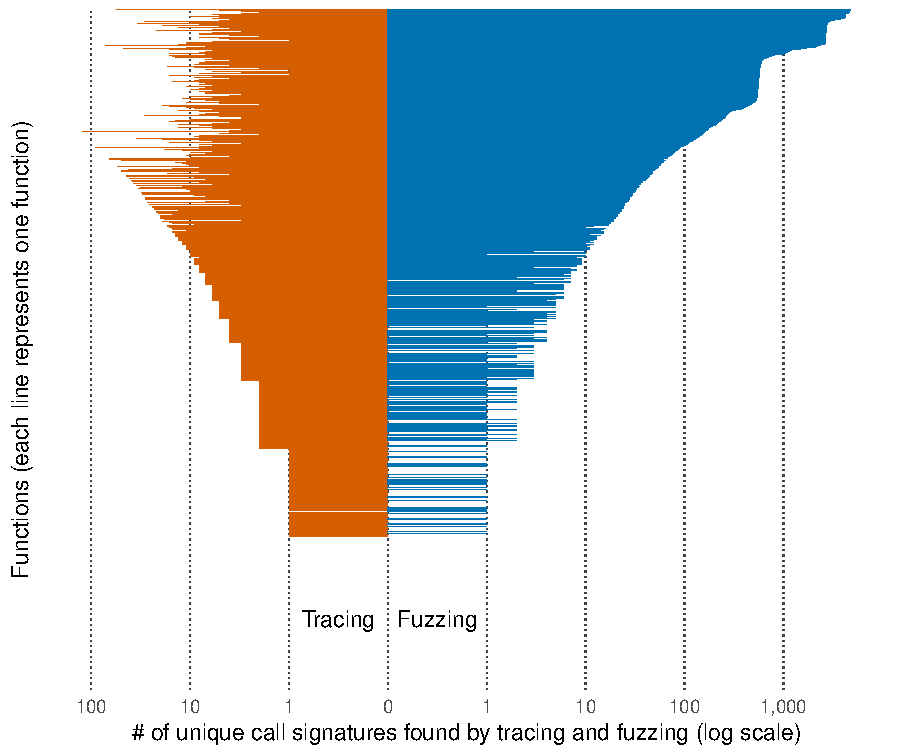
\includegraphics[width=\columnwidth]{code-and-figures/uf-call-signatures.pdf}
    \caption{Number of unique call signatures obtained by tracing and fuzzing. The fuzzer succeeded to generate new calls for \UFNumFunctionsSignatrToCorpusSignatureRatio of the functions in the corpus. The tracer based on the existing code covered \UFNumFunctionsBaselineToCorpusSignatureRatio of the functions.}
    \label{fig:call-signatures}
\end{figure}

\section{Conclusions and Future Work}
\label{sec:conclusions}

Fuzz testing is an incredibly useful technique for finding bugs and security vulnerabilities in code, but is hindered by the permissive semantics of dynamic languages as well as the dynamic nature of how complex data is defined.
In this work, we proposed a fuzzing approach that relies on a database of observed values to provide complex and realistic inputs for functions.
We implement this approach in a tool called \tool for the R programming language, and show that \tool uncovers many new and interesting call signatures for R functions.

While this approach was implemented in a tool for R, it is broadly applicable in all languages, and the only real language-specific aspect is the set of parameters in the database.
For instance, one could implement a similar tool for object-oriented languages, where database metadata could include object field names (\Eg, JavaScript).

%%
%% The next two lines define the bibliography style to be used, and
%% the bibliography file.
\bibliographystyle{ACM-Reference-Format}
\bibliography{fuzzing}

\appendix

\section{\tool demonstration}\label{sec:demo}

The following is a short demo of the basic \tool functionality, \Ie how to create the value database by running R code and then use it to fuzz function type traces.
We will be using the command line interface but the same is available directly in R and thus directly usable from pipeline frameworks such as targets.

\FK{Once I have it up and running I will split the listings into multiple, fix the new lines and add the description to each of the command.}

\begin{lstlisting}
$ cat example-1.R
...

$ cat example-2.R
...

$ ls example*.R | parallel signatr record --from '{1}' --db '{1.-sxpdb}'
...

$ ls -l
...

$ signatr sxpdb-info example-1-sxpdb
...

$ signatr sxpdb-info example-2-sxpdb
...

$ signatr sxpdb-merge --output merged-sxpdb example-*-sxpdb
...

$ signatr sxpdb-info merged-sxpdb
...

$ signatr fuzz --target "base:::`+`" --db merged-sxpdb --budget 100 --output traces
...

$ ls -lh fuzz
...

$ signatr type --traces traces --output types.csv
...

$ wc -l types.csv
...

$ head -10 types.csv
...

$ R -e 'read.csv("type.csv")["signature"] |> unique |> length'
...

\end{lstlisting}

\end{document}
\endinput
